\section{Breve introducción a Docker y contenedores}

Lo que proporcionan los contenedores es un entorno seguro donde nuestra máquina puede correr prgramas.

Podemos lanzar \textit{namespace} y este nos lanza un entorno en el que nos manda a nuestra raíz, de manera que tenemos un filesystem para nosotros. De esta forma tenemos un filesystem aislado. Si ejecutamos \micode{ps -ax} vemos que no vemos los procesos de la máquina anfitriona.   

La idea principal de las redes en los contenedores es que s puedan comunicar entre sí.

En resumen, los contenedores nos dan un espacio aislado y virtualizado. Hay un poco de pérdida de las prestaciones cuando se ejecuta el servicio de red virtualizado, pero es muy poco. Lo mas importante es que el acceso a memoria, CPU, ... son las mismas.

La principal utilización de los contenedores es porque te ofrece un espacio de safe box, y un espacio importante que es el \textit{filesystem privado}. 

Cuando se ejecuta en otros espacios se arrastran todas las dependencias.

Se puede extraer tanto la arquitectura como el sistema operativo, dependencias y demás.

Si necesito un analizador de red, puedo instalarlo sobre un docker y de esta manera no me ensucia mi espacio de trabajo y cuando necesito espacio puedo borrarlo.

En el caso de linux, todos los dockers son sistemas más pequeños sobre linux, con lo básico para que arranque.

Las aplicaciones que ejecutamos en el docker deben de ser ajustadas para que se ejcuten, debido a que la tecnología de docker es diferente a la de la máquina anfitriona.

Debemos de adaptarlo para que pregunte al contenedor por el límtie de aplicaciones que pueden ejecutar, para que todo se ejecute de la manera correcta.

\subsubsection*{Instalación de Docker}

Estan desarrolladas para Linux, por lo que no se puede correr en tecnologías de Windows, si se puede con las extensiones de Linux para Windows.

Usamos la guía de CentOs para instalarlo en Rocky, debemos de tener cuidado con la guía ya que en el último paso, aparecen pasos opcionales para que el docker sea ejecutado sin ser root (privilegios de superusuario).

Podemos instalar el DockerDesktop para un uso más sencillo, pero no es recomendable para un uso profesional.

Se puede ejecuatar sobre MacOs pero usando una máquina virtual, lo cual no tiene mucho sentido.

Entramos en \micode{docker-hub.com}, y buscamos el contenedor de \micode{hello-world}, ya que es el inicial para ver que todo funciona correctamente. Para ello debemos de ejuctar el comando \micode{docker pull hello-world}. Si no indicamos el número de versión, se instala la latest(última versión).

Lo ejecutamos con el comando \micode{docker run hello-world}. Una vez que ejecutamos el comando, se descarga la imagen y se ejecuta el contenedor, mostrando un mensaje para ver que todo ha funcionado correctamente.

\textbf{Todos los ejercicios son opcionales}.

A continuación debemos de centrarnos en el punto de OpenBenchMarking, que es un benchmarking de docker.

El de \micode{blender} es muy utilizado por marcas más comerciales para la renderización de imágenes y vídeos.

Debemos de tener en cuenta siempre las dependencias que necesitamos para ejecutar el contenedor.

Hay una aplicicación que se llama \micode{Phoronix}, que es un benchmarking de docker, pero para el Departamento de ISE, estan pensando en que esta en desuso.

Así que vamos a trabajar con Phoronix en un contenedor para que sea más sencillo de instalar y de ejecutar.

En la guía si buscamos Phoronix, bajamos el de \micode{pts}. Para ello ejecutamos el comando \micode{docker pull phoronix/pts}.

Con el comando \micode{docker images} vemos que se ha descargado la imagen.

SI ejecutamos el comando \micode{docker run -it phoronix/pts} (usamos el comando -it para que se ejecute en el primer plano y os dé una shell interactiva). Con el comando \micode{system-info}, podemos ver las información de los cores, incluso de los que están el un contenedor.

Con el comando \micode{system-sensors}, podemos ver los sensores que el ordenador tiene de manera nativa.

El comando \micode{phoronix-test-suite}(no es que sea un comando es lo que se muestra en la shell cuando ejecutamos el comando anterior de run), y si de seguido añadimos list-available-tests, podemos ver los test que podemos ejecutar. Para más info podemos acceder a la web de docker y en el apartado de dcoumentación.





\subsection*{Apache Benchmark}

Sirve para servidores http. Usando el comando \micode{ab} nos sale la información sobre el mismo. Algunos de los parámetros pueden ser:
\begin{itemize}
    \item -n: Número de peticiones.
    \item -c: Número de conexiones concurrentes.
    \item ...
\end{itemize}

Si lo hacemos con la ugr, podemos ver que en las características que el docuemnto html de la web aparece con muy pocos bytes. Probamos a ejecutar \micode{curl -v http://www.ugr.es}. En específico, \micode{curl} se usa para hacer peticiones http y depurar las mismas. \textit{Debemos de aprender a usarla}.

Vemos que la web de la ugr esta sobre https, por lo que apache-benchmark no se ha dado cuenta, por lo que debemos de usar el comando \micode{ab -n 20 -c 4 https://www.ugr.es/} (debemos de incluir la barra del final) y vemos que en este caso los bytes del html es mucho mayor y es más realista (previamente hemos ejecutado el comando \micode{curl -v http://www.ugr.es/}).



\subsection*{Simulación de Carga con Jmeter}

Se menciona como una tecnología a conocer en las entrevistas de trabajo, por lo que es importante conocerla. 

Usa Java, por lo que podemos usarlo con la última versión de Java.

La lanzamos en 2º plano para que no consuma la consola. Para ello ejecutamos el comando \micode{jmeter &}.

\begin{enumerate}
    \item Añadimos un elemento de thread, que corresponde con las hebras que se van a lanzar de manera concurrente. Para ello pulsamos add y seleccionamos thread group. Añadimos un nombre, hay parámetros que son importatantes. \textit{Se recomienda poner el Jmeter en Inglés para que no haya problemas con los nombres de los elementos y para que las guías de ayuda no tengan errores}. 
    \item Dentro del grupo de hebras creamos un \textit{sample}. Una de las ventajas de Apache es la gran inmensidad de plugins que tiene.  Dentro de sample seleccionamos la \textit{carga de http}. Gracias a la opción de \textit{follow redirects} hace que se ejecute redirecciones de manera automática.
    \item Configuramos los parámetros, como es el prorocolo que vamos a usar, puerto, ...
    \item Añadimos un \textit{listener} para poder ver los resultados (View Results Tree).Para desactivar un elemento debemos de hacer clic derecho y seleccionar la ocpión ``disable''. Hay plugins para poder ver los resultados de manera más visual.
\end{enumerate}

Si queremos simular que se diriga a una página secundaria (ugr.es/centros), debemos de añadir el nombre de la página en el campo de \textit{path}.
Podemos configurar el elmento común de\textit{ HTTP defaults}.

Podemos usar variables de usuario.
Podemos cargar el archivo que nos da bien con la extensión .jtl y usamos jmeter o con un excel (ya que es un archivo en formato csv). 

En cuanto a la aplicación de jmeter, debemos de tener en cuenta que en el order que aparezcan los elementos es el orden en el que se van a ejecutar.

Dentro de /var/logs, tenemos el archivo que muestra los logs y tiene una línea por cada usuario.

El usar el \textit{not sampler} es la forma más habitual de hacerlo, ya que es la forma más sencilla de hacerlo.

\subsection*{Instalación de la aplicación para el test con JMeter}

La aplicación que utilizaremos para el ejercicio de prueba de carga se encuentra en el repositorio de GitHub: \url{https://github.com/davidPalomar-ugr/iseP4JMeter.git}. 

Puede clonar el repositorio utilizando GIT o descargarlo como un archivo comprimido. Una vez descargado, obtendrá un nuevo directorio llamado \texttt{iseP4JMeter}, al cual podrá acceder y levantar la aplicación con los siguientes comandos:

\begin{verbatim}
cd iseP4JMeter
docker compose up
\end{verbatim}

El servicio se lanza en primer plano mostrando los logs de ejecución de sus componentes (incluidas las llamadas HTTP), lo que puede ser muy útil para depurar incidencias. Si desea que el servicio continúe en segundo plano, puede ejecutar el comando con la opción \texttt{-d}:

\begin{verbatim}
docker compose up -d
\end{verbatim}

\subsection*{Detalles sobre el Dockerfile y Docker Compose}

El \texttt{Dockerfile} es el archivo donde se especifican todos los comandos necesarios para crear una imagen de Docker y las acciones que debe realizar sobre esta (como copiar archivos, instalar paquetes o modificar configuraciones). Desde un punto de vista abstracto, podríamos decir que es el \textit{playbook} que Docker aplica al levantar el contenedor.

En este caso, la aplicación sobre la que aplicaremos la carga consta de dos contenedores configurados con sus respectivos \texttt{Dockerfile}s:

\subsubsection*{Dockerfile de la aplicación (Node.js):}

\begin{verbatim}
FROM node:16.13.0-stretch
RUN mkdir -p /usr/src/app
COPY . /usr/src/app
EXPOSE 3000
WORKDIR /usr/src/app
RUN ["npm", "install"]
ENV NODE_ENV=production
CMD ["npm", "start"]
\end{verbatim}

En este archivo se especifica:
\begin{itemize}
    \item La imagen base (\texttt{node:16.13.0-stretch}), que incluye Node.js versión 16.13.0 y Debian Stretch como sistema operativo base.
    \item La creación de un directorio y la copia de los archivos del repositorio en el contenedor.
    \item La exposición del puerto 3000 para la aplicación.
    \item La instalación de las dependencias con \texttt{npm install}.
    \item La ejecución de la aplicación con \texttt{npm start}.
\end{itemize}

\subsubsection*{Dockerfile de la base de datos (MongoDB):}

\begin{verbatim}
FROM mongo:6
COPY ./scripts/* /tmp/
RUN chmod 755 /tmp/initializeMongoDB.sh
WORKDIR /tmp
CMD ./initializeMongoDB.sh
\end{verbatim}

En este archivo se especifica:
\begin{itemize}
    \item La imagen base (\texttt{mongo:6}).
    \item La copia de scripts al contenedor y la asignación de permisos de ejecución.
    \item La ejecución de un script para inicializar la base de datos.
\end{itemize}

\subsubsection*{Archivo \texttt{docker-compose.yml}:}

El archivo \texttt{docker-compose.yml} permite configurar varios contenedores para que trabajen juntos como un único servicio. Su contenido es el siguiente:

\begin{verbatim}
version: '2.0'
services:
  mongodb:
    image: mongo:6
    ports:
      - "27017:27017"
  mongodbinit:
    build: ./mongodb
    links:
      - mongodb
  nodejs:
    build: ./nodejs
    ports:
      - "3000:3000"
    links:
      - mongodb
\end{verbatim}

Este archivo define:
\begin{itemize}
    \item El servicio de MongoDB, exponiendo el puerto 27017.
    \item La inicialización de MongoDB con datos mediante un contenedor adicional.
    \item El servicio de la aplicación Node.js, exponiendo el puerto 3000 y enlazándolo con MongoDB.
\end{itemize}

Para más detalles, consulte la documentación oficial de Docker Compose.

\subsection*{Ejercicio Obligatorio: Simulación de Carga HTTP con JMeter}

El repositorio \url{https://github.com/davidPalomar-ugr/iseP4JMeter.git} contiene la aplicación objeto de la prueba de carga y una descripción de los requerimientos sobre la carga a simular. Siga las instrucciones del repositorio y elabore la prueba de carga con JMeter.

El ejercicio debe realizarse en un directorio que contenga todos los artefactos necesarios para la ejecución de la prueba de carga. Los \textit{paths} a los archivos deben definirse de forma relativa para garantizar que la ejecución sea independiente de la ubicación del directorio. 

Como validación final, debe ser capaz de ejecutar la prueba de carga desde la línea de comandos (sin interfaz gráfica) desde cualquier directorio de su equipo.

\textit{Dentro de la web donde se encuentra la información del ejercicio se nos va indicando lo que debemos de ir haciendo.}

Cuando usamos la API, debemos de tener cuidado con los espacios para evitar errores, además cada alumno solo puede consultar su propio expediente.

Nos vamos a donde hemos clonado el repositorio y ejecutamos el comando \micode{./pruebaEntorno.sh}. 

Para los carácteres extraños que no codifica adecuadamente las webs, podemos usar webs como \textit{urlencoder} para ver como sería codíficado, por ejemplo ``\_'' es ``\%40''

Cuando ejecutmos el comando anterior de \micode{./pruebaEntorno.sh}, se lista varios elementos como es el token que están separados mediante ``.''.

Usando webs como JWT Decoder, si copiamos y pegamos el token aquí, podemos ver la información que contiene. Si mantenemos el ratón en el tiempo de expiración, podemos ver la fecha y hora de expiración. 

Como no se proporciona seguridad, en términos de que cualquiera puede interceptar el token, se nos da un número que representa al usuario en vez del correo (el token si está firmado con la llave), es decir, no esta cifrado pero sí firmado, por ende, podemos ver si lo ha firmado una entidad de confianza.

En cuanto al uso de la herramienta aleatoria, lo relacionado con esto no será materia evaluable. 

\begin{enumerate}
  \item Debemos de crear en Jmeter:
  \begin{itemize}
    \item Thread Group.
    \item Alumnos.
    \begin{itemize}
      \item Dentro de este debemos de crear un HTTP Request y añadirle login y passwd (será de tipo ``POST''), en cuanto al valor que debemos de añadir es \${login} y \${passwd}.
      \item Creamos un \textit{CSV Data Set Config} para poder cargar los datos de los alumnos.
      \item Ahora añadimos un \micode{Post Prodesador}, y este solamente afecta al login.
      \item Luego, añadimos un archivo ``Extraer JWT''. Cuando editamos el archivo, debemos de añadir la variable correspondiente y el campo de valor pasarle el token: ``\${TOKEN}''.
    \end{itemize}
  \end{itemize}
  \item Creamos las variables que se indican con TestPlan.
\end{enumerate}
\textit{Básicamente debemos de leernos la documentación para poder realizar la práctica.}

Los documentos que debemos de tener según las clases de teoría son:

\begin{figure}[H]
  \centering
  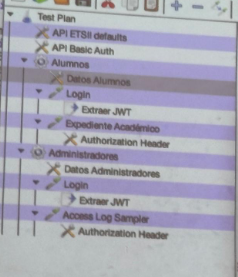
\includegraphics[width=0.8\textwidth]{images/Bloque2/docs_clase_jmeter.png}
  \caption{Documentos necesarios para la práctica.}
  \label{fig:documentos_practica}
\end{figure}

Debemos de entregar en Prado los archivos de carga ya que lo demás lo tiene él.

\subsection*{Docker Compose}

Docker Compose es una herramienta que permite definir y ejecutar aplicaciones Docker de múltiples contenedores. Con Compose, puedes usar un archivo YAML para configurar los servicios de tu aplicación, y luego con un solo comando puedes crear e iniciar todos los servicios desde esa configuración, este lee nuestro archivo \texttt{docker-compose.yml} y levanta los contenedores según la configuración especificada.

Entramos en \micode{hub.docker.com} y buscamos \micode{mongo:6} la imagen es un cuadrado\footnote{El link es \url{https://hub.docker.com/r/litmuschaos/mongo}.}. Ya solo queda entrar en el docker y ejecutar ese contenedor de manera independiente haciendo uso del comando \micode{docker run -it mongo:6}.

En el Docker Compose no necesitamos el mapeado de puertos. 

Si entramos en el directorio mongodb y abrimos el archivo dockerfile\footnote{Es similar a un makefile.} y lo ejecutamos, se nos crea un contenedor de mongo, vemos que ejecuta el archivo init.db, inicializando la base de datos con los datos que esten ahí definidos. Una imagen se basa en otra y así hasta que al final se llega a la imagen de linux.  


\section{Monitoring}

\subsection*{Top}

Para ejecutarlo en nuestra máquina debemos de ejecutar el comando \micode{top}. Este comando nos muestra los procesos que se están ejecutando en la máquina, junto con información sobre el uso de CPU, memoria y otros recursos.

Si ejecutamos el comando \micode{more loadavg}, nos ofrece en cada momentos el valor de los programas, tiempo de ejecución, etc.

El comando \micode{wath -n <tiempo> <"comando">}, de esta manera nos ejecuta el comando que se expone cada <tiempo> segundos.

Si vemos en una máquina con un solo core vemos un 1, quiere decir, que siempre había un proceso esperado para ejecutarse, es decir, que la CPU esta saturada, el uso de la CPU es del 200\%.

Si tenemos un 1 y 2 cores, significa que la CPU está al 50\%, es decir, que no está saturada.

Si tenemos 4 cores y tenemos un 4, significa que la CPU está al 100\%.

\subsection*{Información de Top en Linux}

El comando \texttt{top} en Linux muestra información en tiempo real sobre los procesos en ejecución y el estado del sistema. A continuación, se explica el significado de cada elemento que aparece en su salida:

\subsubsection*{Encabezado del sistema (primeras líneas)}

Este bloque muestra información general del sistema.

\paragraph{Primera línea: Tiempos de actividad}
\begin{verbatim}
top - 16:35:28 up 2:15,  2 users,  load average: 1.23, 0.85, 0.67
\end{verbatim}
\begin{itemize}
  \item \textbf{16:35:28}: Hora actual del sistema.
  \item \textbf{up 2:15}: Tiempo que el sistema lleva encendido (en este caso, 2 horas y 15 minutos).
  \item \textbf{2 users}: Número de usuarios conectados.
  \item \textbf{load average: 1.23, 0.85, 0.67}: Promedio de carga del sistema en los últimos 1, 5 y 15 minutos. Valores cercanos o superiores al número de núcleos indican alta carga.
\end{itemize}

\paragraph{Segunda línea: Tareas en ejecución}
\begin{verbatim}
Tasks: 180 total, 2 running, 177 sleeping, 1 stopped, 0 zombie
\end{verbatim}
\begin{itemize}
  \item \textbf{180 total}: Número total de procesos.
  \item \textbf{2 running}: Procesos que están ejecutándose activamente.
  \item \textbf{177 sleeping}: Procesos en espera de eventos.
  \item \textbf{1 stopped}: Procesos detenidos (pausados).
  \item \textbf{0 zombie}: Procesos "zombie" (terminados pero aún en la tabla de procesos).
\end{itemize}

\paragraph{Tercera línea: Uso de CPU}
\begin{verbatim}
%Cpu(s):  3.5 us,  1.2 sy,  0.0 ni, 95.0 id,  0.2 wa,  0.0 hi,  0.1 si,  0.0 st
\end{verbatim}
\begin{itemize}
  \item \textbf{us (user)}: \% de CPU utilizado por procesos de usuario.
  \item \textbf{sy (system)}: \% de CPU utilizado por procesos del sistema (kernel).
  \item \textbf{ni (nice)}: \% de CPU consumido por procesos con prioridad ajustada (\texttt{nice}).
  \item \textbf{id (idle)}: \% de CPU inactiva.
  \item \textbf{wa (I/O wait)}: \% de CPU esperando operaciones de entrada/salida (disco, red).
  \item \textbf{hi (hardware interrupts)}:\% de CPU manejando interrupciones de hardware.
  \item \textbf{si (software interrupts)}: \% de CPU manejando interrupciones de software.
  \item \textbf{st (steal time)}: \% de CPU "robado" por una máquina virtual (si se ejecuta en un entorno virtualizado).
\end{itemize}

\paragraph{Cuarta y quinta líneas: Uso de memoria RAM y Swap}
\begin{verbatim}
MiB Mem :   7854.2 total,   2364.5 free,   3184.8 used,   1304.9 buff/cache
MiB Swap:   2048.0 total,   1024.0 free,   1024.0 used.  2345.6 avail Mem
\end{verbatim}
\begin{itemize}
  \item \textbf{Mem total}: Memoria RAM total del sistema.
  \item \textbf{free}: Memoria libre disponible.
  \item \textbf{used}: Memoria en uso.
  \item \textbf{buff/cache}: Memoria usada como caché y buffers.
  \item \textbf{Swap total}: Tamaño total del área de intercambio (swap).
  \item \textbf{Swap free}: Espacio de swap no utilizado.
  \item \textbf{Swap used}: Espacio de swap en uso.
  \item \textbf{avail Mem}: Memoria disponible para nuevas aplicaciones.
\end{itemize}

\subsubsection*{Lista de procesos}

Esta sección muestra información sobre los procesos en ejecución. Cada columna tiene un significado:

\begin{verbatim}
PID   USER      PR  NI    VIRT    RES    SHR S  %CPU %MEM     TIME+ COMMAND
\end{verbatim}

\paragraph{Columnas principales}
\begin{itemize}
  \item \textbf{PID}: Identificador único del proceso.
  \item \textbf{USER}: Usuario que ejecuta el proceso.
  \item \textbf{PR (priority)}: Prioridad del proceso.
  \item \textbf{NI (nice)}: Valor \texttt{nice}, afecta la prioridad del proceso (-20 = más prioridad, 19 = menos prioridad).
  \item \textbf{VIRT (virtual memory)}: Memoria virtual utilizada (RAM + swap).
  \item \textbf{RES (resident memory)}: Memoria RAM utilizada sin contar swap.
  \item \textbf{SHR (shared memory)}: Memoria compartida con otros procesos.
  \item \textbf{S (state)}: Estado del proceso:
  \begin{itemize}
    \item \texttt{R}: Running (ejecutándose).
    \item \texttt{S}: Sleeping (durmiendo).
    \item \texttt{D}: Uninterruptible sleep (espera de I/O).
    \item \texttt{T}: Stopped (detenido).
    \item \texttt{Z}: Zombie (proceso finalizado, pero aún listado).
  \end{itemize}
  \item \textbf{\%CPU}: Porcentaje de uso de CPU del proceso.
  \item \textbf{\%MEM}: Porcentaje de uso de RAM del proceso.
  \item \textbf{TIME+}: Tiempo total de CPU consumido por el proceso.
  \item \textbf{COMMAND}: Comando o nombre del proceso.
\end{itemize}

\subsubsection*{Atajos útiles en \texttt{top}}

\begin{itemize}
  \item \texttt{q}: Salir de \texttt{top}.
  \item \texttt{h}: Mostrar ayuda.
  \item \texttt{k}: Matar un proceso (requiere PID).
  \item \texttt{M}: Ordenar por uso de memoria.
  \item \texttt{P}: Ordenar por uso de CPU.
  \item \texttt{T}: Ordenar por tiempo de ejecución.
\end{itemize}


Si entramos en el directorio /proc/sys/net/ipv4, podemos ver los parámetros de configuración del kernel.

Además del comando \micode{uptime}, podemos usar el comando free, que nos muestra la memoria libre y ocupada. Si usamos el comando \micode{free -h}, nos muestra la información en un formato más legible (human readable). Una de las ventajas de estos comandos es que no es interactivo, es decir, que ocupan la terminal, como si lo es el comando \micode{top}. Además, podemos usar el comando \micode{vmstat}.

El comando \micode{stress} se usa para generar pruebas artificiales sobre el uso de memoria y demás.

Si usamos \micode{htop}, es una versión mejorada de \micode{top} y nos muestra la información de una manera más visual. Para instalarlo, usamos el comando \micode{apt install htop}. Si lo ejecutamos, vemos que se nos muestra la información de una manera más visual.

\section{Cron}

Este se define como un demonio que se encarga de ejecutar tareas programadas en el sistema. Se utiliza para automatizar tareas repetitivas, como copias de seguridad, actualizaciones de software y mantenimiento del sistema. Podemos usar herramientas externas como \url{https://freeformatter.com}, para que nos de la configuración del crontab traduciendo para ello la expresión cron. Una alternativa a cron es \micode{anacron}. Este se ejecuta por defecto una vez cada hora.

Debemos de aprender a manejar el comando \micode{journalctl}. Si usamos \micode{journalctl -f}, nos muestra los logs en tiempo real. Si usamos \micode{journalctl -u cron}, nos muestra los logs del servicio de cron. Si usamos \micode{journalctl -u cron --since "2023-10-01 12:00:00"}, nos muestra los logs desde esa fecha y hora, tenemos una gran infinidad de opciones para filtrar los logs\footnote{Para ello podemos entrar en la documentación oficial.}. Cuando reiniciamos el equipo, perdemos los mensajes de logs de ayer, por lo que debemos de tener cuidado con esto. Para habilitarlo debemos de entrar en /etc/systemd/journald.conf y cambiar el parámetro de Storage de auto a yes, descomentando la línea. 

El programa \micode{logrotate} se encarga de gestionar los logs, y lo podemos encontrar en /etc/logrotate.conf. Este programa se encarga de rotar los logs, es decir, de crear un nuevo log y eliminar el antiguo. Si no lo tenemos configurado, los logs pueden ocupar mucho espacio en disco. Dentro de logrotate.d podemos añadir archivos de configuración para cada uno de los logs.


\section{Grafana + Prometheus}

Prometheus es el encargado de preguntarle a cada nodo por sus métricas, este proceso se llama \textbf{scraping}. Lo que almacena son series temporales mediante muestreos que realiza cada cierto tiempo. Puede presentar una interfaz de usuario, pero esta es muy pobre.

Una alternativa de usar la BD de Prometheus es \textit{InfluxDB} que es una opción de BD más rápida.

Vamos a usar la que tiene Grafana mediante en lenguaje de\textit{ PromQL}, en el cual se dibujan diagramas, alertas y demás.

Tenemos lo que se conoce como \textit{exporters} que son las interfaces web que va a llamar Prometheus.

Para acceder a la web de Prometheus debemos de acceder al enlace: \url{https://prometheus.io/}.

Debemos de conocer Counter, Cauge e Histogram.

Para empezar a hacer el ejercicio dentro del guión tenemos dos archivos, copiamos el contenido de los dos archivos de compose y de Prometheus. 

\begin{lstlisting}[style=yamlstyle]
  docker-compose.yml:
---
version: "3"
services: # usamos dos servicios
prometheus:
image: prom/prometheus:v2.50.0
ports:
- 9090:9090 # es el puerto de Prometheus
volumes:
- ./prometheus_data:/prometheus # aquí almacena todos sus datos y lo mapeamos en un directorio externo, de manera que los cambios que realicemos aquí se guardan de manera permanente.
- ./prometheus.yml:/etc/prometheus/prometheus.yml # lo almacena dentro de el directorio /etc correspondiente a la configuración de Prometheus, estamos montando un volumen.
command:
- "--config.file=/etc/prometheus/prometheus.yml"
grafana:
image: grafana/grafana:9.1.0
ports:
- 4000:3000 # el puerto estandar es el 3000, pero es el mismo de node, para que no haya colisión, debemos de mapearlo sobre el 4000
volumes:
- ./grafana_data:/var/lib/grafana
depends_on:
- prometheus
\end{lstlisting}

Lo arrancamos como siempre con \micode{docker compose up}, una vez que sepamos que funciona lo arrancamos en 2º plano para saltarnos todos los logs que aparecen. Cuando lo lanzamos se nos crean dos subdirectorios, la de Grafana y la de Prometheus, si queremos resetarlos borramos estos dos directorios, ya que estos son los que almacenan el estado.

\begin{lstlisting}[style=yamlstyle]
  prometheus.yml:
---
global:
scrape_interval: 5s # el tiempo en el que le pregunta por sus metricas
scrape_configs:
- job_name: "prometheus_service" # el nombre del servicio, es decir, Prometheus se esta monitorizando a sí mismo.
static_configs: # de esta manera le estamos diciendo donde se encuentra el nombre de Prometheus.
- targets: ["prometheus:9090"]
\end{lstlisting}

Dentro de la web de Prometheus debemos de entrar en targets para depurar el código, cada uno de los exporters que aparecen si esta en verde es que esta \textcolor{green}{correcto}.

Para las consultas, vamos a la parte gráfica (Status/Targets). Si accedemos a la dirección de Prometheus nos da error porque solo tiene sentido dentro del docker compose, por ende, debemos de cambiar a localhost y lo que sigue.

Una de las grandes ventajas de los exporters es la sencillez al usar texto plano.

No podemos usar safari debido a que no esta soportado correctamente con grafana y Prometheus.

En el ejercicio que nos pide, vamos a usar poco los labels, se van a usar más cuando hagamos la API el Jmeter, pero en general, se usan pocos, se copian las métricas,se deben de copiar completamente.

Hay una función muy importante que vamos a usar mucho dentro de Prometheus, \textbf{rate}.

Este comando \micode{rate(http_requests_total{job="api-server"}[5m])}.

\subsubsection*{Significado paso a paso:}

\begin{itemize}
  \item \texttt{http\_requests\_total\{job="api-server"\}}:
  \begin{itemize}
    \item Selecciona la métrica \texttt{http\_requests\_total}, que suele ser un contador del número total de peticiones HTTP.
    \item El filtro \texttt{\{job="api-server"\}} indica que solo se quieren las métricas donde la etiqueta \texttt{job} tenga el valor \texttt{"api-server"}. Esto restringe los resultados a esa parte del sistema.
  \end{itemize}
  \item \texttt{[5m]}:
  \begin{itemize}
    \item Es un selector de rango que indica: "mira los últimos 5 minutos de esa serie temporal".
  \end{itemize}
  \item \texttt{rate(...)}:
  \begin{itemize}
    \item La función \texttt{rate()} calcula la tasa de cambio promedio por segundo de una métrica de tipo \textit{counter} dentro del rango de tiempo especificado.
    \item En este caso: "¿a qué velocidad están aumentando las peticiones HTTP por segundo en los últimos 5 minutos?".
  \end{itemize}
\end{itemize}

\subsubsection*{ ¿Qué te devuelve?}

Te da la tasa promedio de solicitudes HTTP por segundo para el \texttt{api-server}, calculada a partir de los datos recogidos en los últimos 5 minutos.

\subsubsection*{ Uso típico:}

Esta consulta se usa comúnmente en dashboards de Grafana o alertas de Prometheus, para ver el ritmo de carga que tiene un servicio web.

Entramos en grafana: \url{https://grafana.com/}

Entramos en Grafana y en Settings/ Data Sources y usamos Prometheus, le damos el puerto y \micode{http://prometheus:9090}.

Ahora debemos de hacer un \textit{Dashboards}, New, New Dashboard, add new panel, seleccionamos labels, y metrics, se recomienda hacer con el builder ya que va sugiriendo. En el campo vacío añadimos el comando rate de antes.

Si nos damos cuenta el resultado de rate es un tanto por 1, por ende, si lo multiplicamos $\times$ 100 nos da un porcentaje, para ello buscamos la opciónn multiplicate. Dentro de la definición del espacio de trabajo podemos ajustar la curvatura de las líneas, el estilo, ejes, ...

También podemos añadir reglas/alertas para que, por ejemplo, cuando llegue al 70\% de CPU que me avise.

\subsection{jercicio Obligatorio. Monitorización con Grafana + Prometheus.}

Dentro de la máquina Rocky debemos de instalar le exporter de Prometheus. Este se puede lanzar por línea de comandos. Debemos de crear un servicio para que cuando se inicie el equipo estén los exporters, y estos publican los puertos HTTP donde se puede hacer scraping.

Este enlace nos ofrece una guía de como hacerlo paso a paso, es decir, un tutorial: \url{https://devopscube.com/monitor-linux-servers-prometheus-node-exporter/}. Si accedemos desde fuera no nos va a dejar, por ende, debemos de habilitar ese puerto en el firewall. Este año debemos de modificar el security extension, ya que si se cae no nos dice nada, en este caso podemos deshabilitarlas (no recomienda), o ejecutar el comando \micode{restorecon -v <donde lo hayamos instalado>}.

Ahora debemos de modificar el siguiente fichero: \micode{prometheus.yml:} y añadimos: 

\begin{lstlisting}[style=yamlstyle]
  - job_name: "node" # se recomienda poner node
static_configs:
- targets: ["IP DE NUESTRA MÁQUINA:9100"]
\end{lstlisting}

Dentro de grafana debemos de copiar el ID, entramos en los dashboard y lo importamos, y copiamos el ID.

\textit{Nota: Debemos de ponerlo node, ya que por defecto es mejor y más sencillo.}

Se recomienda coger el dashboard, vamos al panel y lo fusionamos, esto no es fácil, debemos de preguntarle al profesor.

\textcolor{blue}{\textit{Debemos de entregar un pdf en el que se explique todo al detalle con capturas de pantalla y demás. De la parte de monitores debemos de parar aunque sea 1. Lo más importante es que se vea la gráfica.}}

Dentro de la API web podemos añadir /metrics y vemos las métricas.

Una de las alternativas más rentables es coger todos los contendores del JS y añadirlo dentro del Docker Compose. La mejor sería usar la tarjeta que nos ofrece el propio \textit{docker compose}. No podemos usar la de la IP ya que cada vez que arrancamos la máquina esta cambia al usar una IP dinámica.



